\section{Memoria principale}\label{main memory}
Fino ad ora abbiamo discusso di come un sistema operativo gestisce lo scheduling (\ref{CPU scheduling}), la sincronizzazione (\ref{sincronizzazione}) e i deadlock (\ref{deadlocks}) sorvolando sempre sulla locazione effettiva su cui questi processi vengono mantenuti, ovvero la memoria. Osserviamo sin dall'inizio che con memoria intendiamo la memoria RAM del calcolatore, le memorie secondarie molto capienti sono i dischi e le memorie di massa, che verranno discusse approfonditamente nel capitolo \ref{mass memory}. In particolare in questo capitolo ci occuperemo di dare un'introduzione ai concetti generali, passando poi a discutere il metodo più semplice per risolvere l'utilizzo della memoria, ovvero l'allocazione continua per poi discutere un tecnica più avanzata che tutt'ora si trova nei sistemi operativi moderni, ovvero il \textit{paging}. Scopriremo che saranno necessarie delle strutture ausiliarie, come la tabella delle pagine, e ne studieremo i diversi metodi di implementazione. Infine ci dedicheremo al concetto di \textit{swapping} e a modelli di allocazioni alternativi alla paginazione.

\subsection{Introduzione}
Come sappiamo, il programma, una volta che viene eseguito, deve essere caricato dal disco in memoria. Solo una volta che è stato caricato in memoria può essere eseguito; questo perché la CPU non ha accesso diretto alla memoria di massa. Sappiamo inoltre che l'accesso della CPU è effettuato seguendo 3 tipi di memorie (figura \ref{fig:memory_hierarchy}):
\vspace{-5px}
\begin{itemize}
\setlength{\itemsep}{-.15 em}
    \item Registri, che hanno un accesso rapidissimo;
    \item RAM, che ha una velocità sicuramente ridotta rispetto ai registri;
    \item \textbf{Cache}, che è una piccola memoria che fa da intermediario tra i registri e la RAM ed ha un tempo di accesso molto più veloce della memoria.
\end{itemize}
\begin{figure}[h]
    \centering
    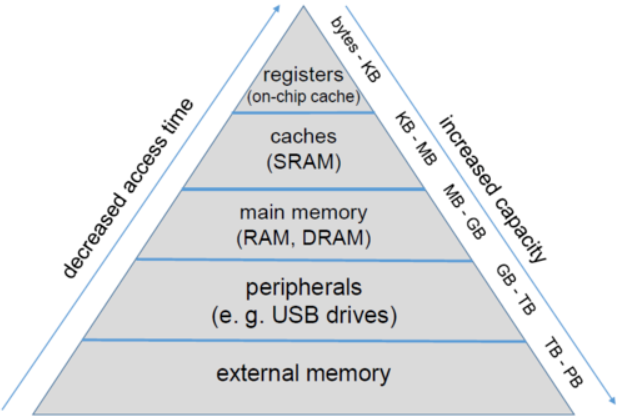
\includegraphics[width = .5\textwidth]{../res/imgs/main memory/memory_hierarchy.png}
    \caption{La gerarchie delle memorie nel calcolatore.}
    \label{fig:memory_hierarchy}
\end{figure}

% 
\subsubsection{Protezione}
In generale, se vogliamo avere molti processi che vengono caricati contemporaneamente nell'area della memoria e che vengono eseguiti in modo concorrente, è importante che ci sia una protezione dei processi fornita dal sistema operativo al fine di garantire che ogni processo abbia il suo spazio di memoria senza che vada a collidere con un altro processo. La soluzione più banale, rappresentata in figura \ref{fig:process_protection}, è quella di utilizzare due registri che tengono traccia di due valore: l'indirizzo \textbf{base}, ovvero l'indirizzo in memoria iniziale da cui il processo parte, e il valore \textbf{limite} (\textit{offset}) che indica la massima espansione del processo in memoria. In altre parole, il processo in memoria non può superare l'indirizzo "base + limite" (più avanti in questo capitolo vedremo soluzione più complesse e raffinate).
\begin{figure}[h]
    \centering
    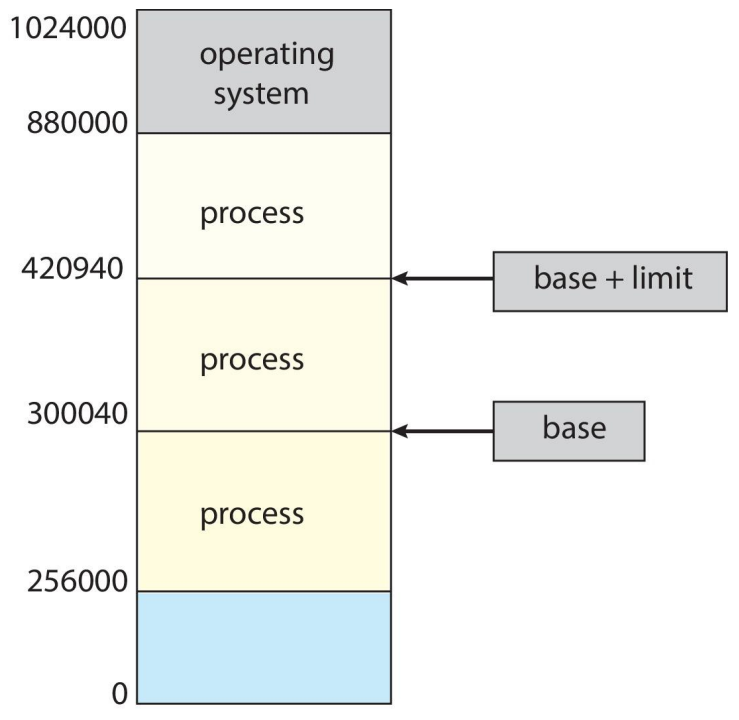
\includegraphics[width = .35\textwidth]{../res/imgs/main memory/process_protection.png}
    \caption{Limite inferiore e limite superiore dello spazio del processo in memoria.}
    \label{fig:process_protection}
\end{figure}
In questo caso l'unica preoccupazione del sistema operativo è controllare, ogni volta che un indirizzo viene generato dalla CPU durante l'esecuzione del programma, se questo indirizzo è compreso tra la base e l'offset fornito dai due registri. Nel caso in cui l'indirizzo è compreso allora la locazione di memoria può essere acceduta. Osserviamo che la figura \ref{fig:can_access} rappresenta un piccolo schema dove viene illustrata questa verifica da parte del sistema operativo.
\begin{figure}[h]
    \centering
    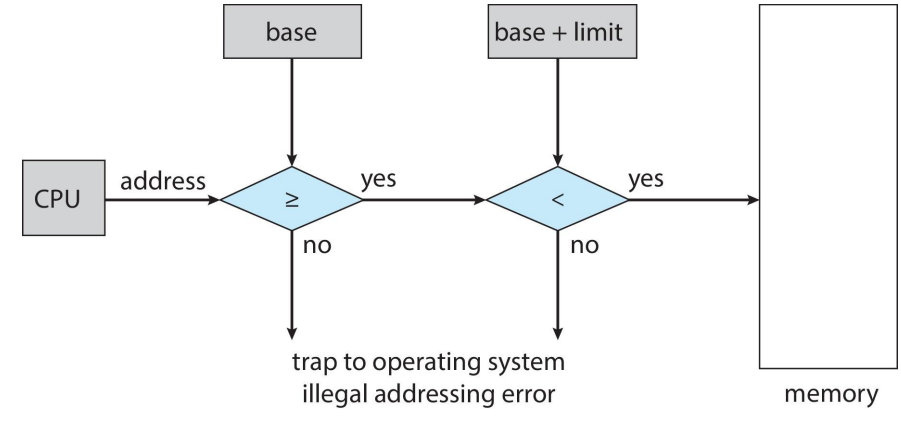
\includegraphics[width = .6\textwidth]{../res/imgs/main memory/can_access.png}
    \caption{Procedura di controllo di un indirizzo mediante il SO.}
    \label{fig:can_access}
\end{figure}

% 
\subsubsection{Binding}
Quando creiamo un processo, di default parte dall'allocazione 0000. Naturalmente non è possibile far partire tutti i processi dalla stessa allocazione altrimenti si genererebbero conflitti che causerebbero problemi non indifferenti. Inoltre ogni processo che viene eseguito, anche se il suo indirizzo in memoria è diverso 0000, viene eseguito come se la sua prima cella disponibile fosse la 0000. Come è possibile? Il procedimento è chiamato \textbf{binding} e mappa due tipi di indirizzi: gli indirizzi \textbf{assoluti}, che sono gli effettivi indirizzi nella memoria, e gli indirizzi \textbf{rilocabili} che sono gli indirizzi relativi al programma in esecuzione. Per chiarire le idee, facciamo un esempio: poniamo di avere un processo che parte dall'indirizzo in memoria \texttt{31400} (indirizzo assoluto) e che stia eseguendo una linea di codice che secondo il processo è all'indirizzo \texttt{15}. In realtà il programma non sta eseguendo l'indirizzo \texttt{15} ma sta eseguendo l'indirizzo assoluto \texttt{31415}, che è la somma tra l'indirizzo fisico di inizio e l'indirizzo logico (31400 + 15). Questa somma, è infatti detta binding e permette di collegare gli indirizzi logici del processo agli indirizzi fisici della memoria. 

\begin{wrapfigure}{o}{.30\textwidth}
  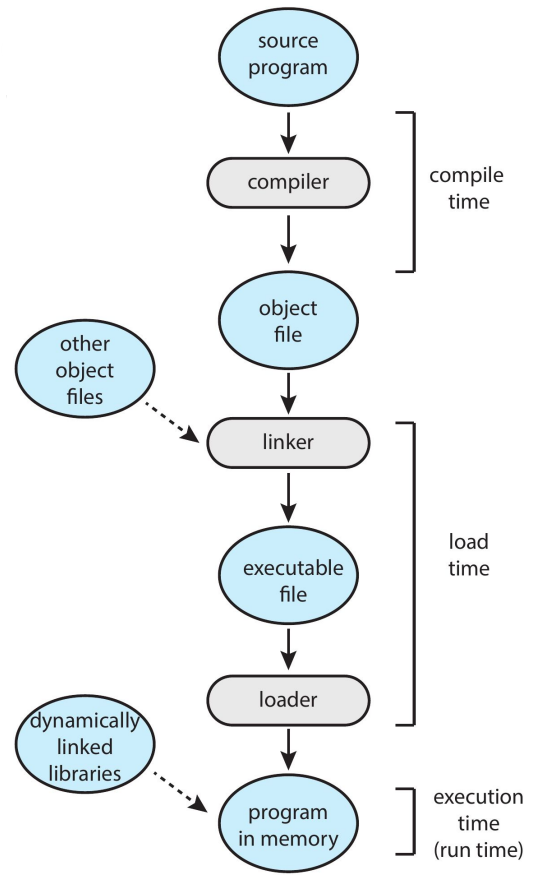
\includegraphics[width = \linewidth]{../res/imgs/main memory/binding_time.png}
  \caption{I tre tempi di binding.}
  \label{fig:binding_time}
\end{wrapfigure}
Il binding però può avvenire in diversi momenti, come è possibile anche osservare dalla figura \ref{fig:binding_time}. Possiamo distinguere principalmente 3 momenti:
\vspace{-5px}
\begin{enumerate}
\setlength{\itemsep}{-.15 em}
    \item Tempo di \textbf{compilazione}: in questo caso, il compilatore, compilando il codice automaticamente converte gli indirizzi rilocabili in indirizzi assoluti.
    \item Tempo di \textbf{caricamento}: nel momento di \textit{linking} del programma e quindi si ha un eseguibile che ha ancora gli indirizzi temporanei ma che poi, una volta caricato, verranno sostituiti con gli indirizzi assoluti.
    \item Tempo di \textbf{esecuzione}: è infine possibile trasformare gli indirizzi rilocabili in indirizzi assoluti durante l'esecuzione del programma. Questo è il metodo tipicamente utilizzato dai sistemi operativi moderni, attraverso tecniche che approfondiremo in questo capitolo.
\end{enumerate}

È quindi fare un'importante distinzione tra due tipi di indirizzi. Lo spazio di indirizzi che è visto dal programma (e quindi è indipendente dalla macchina in cui risiede) è chiamato spazio degli indirizzi \textbf{logici} (o \textbf{virtuali}, come vedremo nel capitolo \ref{virtual memory}). D'altro canto, lo spazio degli indirizzi in memoria, ovvero gli indirizzi assoluti, è chiamato spazio degli indirizzi \textbf{fisici}. 

% 
\subsubsection{Memory-Management Unit (MMU)}
Parte dei meccanismo utilizzati per gestire la memoria e il binding non sono lasciati solamente al sistema operativo ma sono un ibrido tra hardware e software. Questo hardware è detto \textit{Memory-Management Unit} (\textbf{MMU}) ed aiuta a mappare gli indirizzi logici in indirizzi fisici. Questo modulo era originariamente un chip a parte, tra la CPU e la memoria, con l'avanzare del tempo l'MMU è una parte integrata nella CPU stessa.

Una delle funzionalità dell'MMU è quella di fornire il controllo sull'indirizzo del processo nella memoria. È la stessa funzionalità che implementava il sistema operativo (vedi figura \ref{fig:can_access}) solo che in questo caso il controllo è effettuato autonomamente dell'MMU attraverso un particolare registro chiamato \textbf{relocation register}. Il processo è rappresentato nell'illustrazione \ref{fig:can_access_MMU}.

\begin{figure}[h]
    \centering
    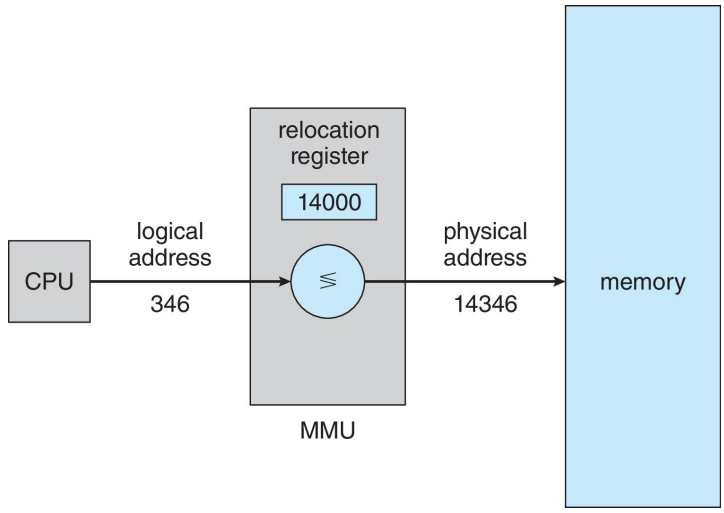
\includegraphics[width = .55\textwidth]{../res/imgs/main memory/can_access_MMU.png}
    \caption{Procedura di controllo di un indirizzo mediante la MMU.}
    \label{fig:can_access_MMU}
\end{figure}

% 
\subsubsection{Caricamento e collegamento dinamico}\label{dynamic loading and linking}
Uno dei concetti fondamentali nell'uso della memoria è il \textbf{dynamic loading}. Ciò significa che dal punto di vista del programma non è possibile mantenere tutte le funzioni necessarie del programma sempre in memoria, ma mantenere solo un sottoinsieme che sono al momento necessarie. Nel momento in cui una nuova routine è necessaria la si va a caricare dalla memoria.

Un secondo approccio è quello del \textit{linking}. In particolare il collegamento può essere fatto in due modi: statico e dinamico. Lo \textbf{static linking} avviene quando colleghiamo le librerie di sistema al programma e una volta compilato il programma le librerie sono immediatamente integrate nel file eseguibile. A questo si contrappone il \textbf{dynamic linking} dove il codice delle librerie non viene caricato nel file eseguibile ma le librerie sono collegate solo durante l'esecuzione del programma. Sono infatti presenti delle \textbf{shared libraries}, come le \texttt{dll} di Windows, che vengono caricate in memoria e condivise a tutti i processi che le necessita e, un volta che nessun processo le utilizza più, queste vengono rimosse dalla memoria. Questo è molto più conveniente rispetto al collegamento statico dove in memoria ci possono essere potenzialmente diversi programmi che hanno una copia della libreria nel codice. Questo significa che la stessa libreria occupa molto più spazio in memoria perché è copiata da diversi processi. Se invece ci fosse stata una librerie dinamica, tutti i processi avrebbero usufruito il codice della stessa in modo tale da risparmiare dello spazio prezioso in memoria.

% 
\subsection{Primi modelli di allocazione}
Passiamo ora a vedere la storia e i concetti della paginazione della memoria per poi arrivare a discutere dei metodi moderni e tuttora utilizzati.

% 
\subsubsection{Allocazione contigua}
La prima soluzione che è stata pensata è l'allocazione contigua (figura \ref{fig:memory_contiguos_allocation}) in memoria: 
\begin{figure}[h]
    \centering
    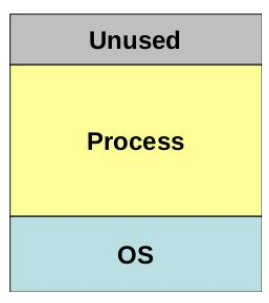
\includegraphics[width = .15\textwidth]{../res/imgs/main memory/contiguos_allocation.png}
    \caption{Allocazione contigua dei processi in memoria.}
    \label{fig:memory_contiguos_allocation}
\end{figure}
ciò significa avere una parte dedicata al sistema operativa (kernell) e poi, in modo contiguo, inizia il codice per i processi.

Il modo più semplice per poter implementare questo meccanismo è attraverso il \textit{limit register} e il \textit{reloction register} che abbiamo visto poco fa. Questo infatti permette di proteggere i processi tra di loro, evitando quindi che si sovrappongano in memoria. Osservando infatti l'illustrazione \ref{fig:relocation_register_allocation} possiamo notare che dalla CPU viene preso l'indirizzo logico (ovvero l'indirizzo relativo per il processo), viene controllato se "sfora" il limite massimo in memoria; una volta che è stato appurato che l'\textit{upper bound} non è stato superato, il relocation register procede con il \textit{binding}.
\begin{figure}[h]
    \centering
    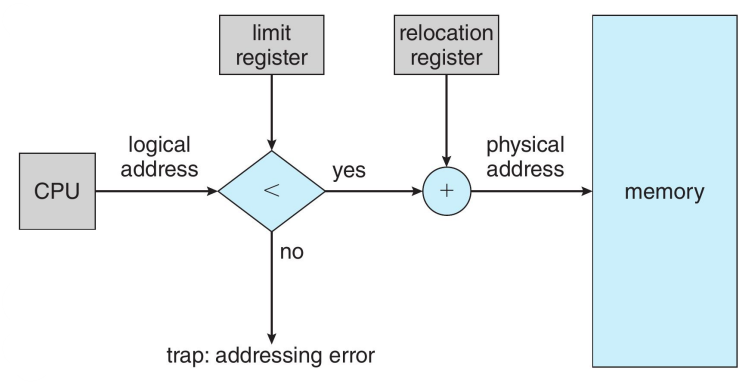
\includegraphics[width = .5\textwidth]{../res/imgs/main memory/relocation_register_allocation.png}
    \caption{I registri utilizzati per il binding tra logico e fisico.}
    \label{fig:relocation_register_allocation}
\end{figure}

% 
\subsubsection{Allocazione a partizione fissa}\label{partizione_fissa}
Un a soluzione un po' più raffinata, è l'allocazione a partizione fisse. Questo tipo di allocazione consiste nel dividere la memoria in un insieme di partizioni di dimensione non variabile e andare ad allocare i processi, non in modo contiguo, ma in una partizione la cui dimensione è adeguata e consona alla dimensione del processo. 
\begin{figure}[h]
    \centering
    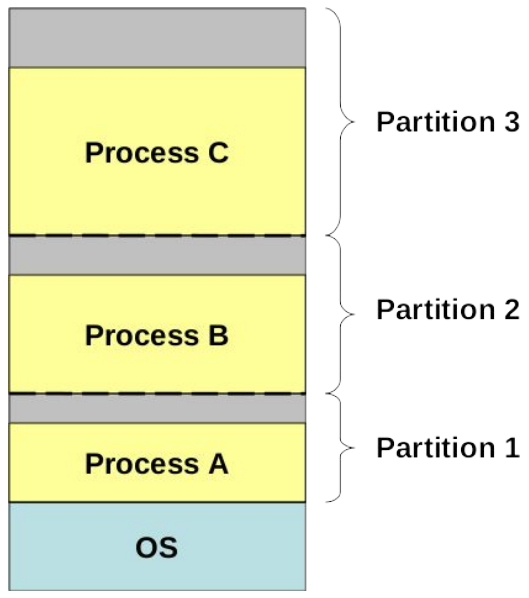
\includegraphics[width = .28\textwidth]{../res/imgs/main memory/fixed_partition.png}
    \caption{La memoria divisa in partizioni fisse per i processi.}
    \label{fig:fixed_partition}
\end{figure}
Osservando la figura \ref{fig:fixed_partition} notiamo che, innanzitutto le partizioni possono essere di dimensione diversa (l'importante è che non cambi nel tempo) al fine di gestire processi si dimensione diversa. Notiamo già i possibili problemi di questo tipo di modello, primo tra tutti è lo spazio in memoria inutilizzato grigio alla fine di ogni partizione (vedi il paragrafo \ref{frammentazione}: frammentazione interna). L'idea però della partizioni fisse è un concetto che, come vedremo verrà ripreso nella paginazione (paragrafo \ref{paginazione}), presente nei sistemi operativi moderni.

% 
\subsubsection{Allocazione a partizione variabile}\label{partizione_variaibile}
In alternativa alla partizione fissa, possiamo avere un tipo di allocazione in cui la dimensione della partizione varia a seconda del processo che fa richiesta. Osservando l'illustrazione \ref{fig:variable_partition} notiamo che il processo 8, una volta che è terminato lascia un buco ad un secondo processo, il 9 che però occupa meno spazio, di conseguenza la dimensione della partizione è variata.
\begin{figure}[h]
    \centering
    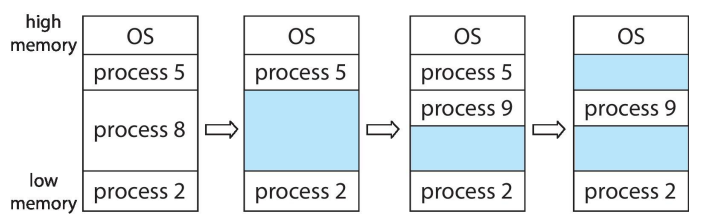
\includegraphics[width = .55\textwidth]{../res/imgs/main memory/variable_partition.png}
    \caption{Rappresentazione di una partizione variabile in memoria.}
    \label{fig:variable_partition}
\end{figure}
Anche in questo caso, come nella partizione fissa, si può incombere in una frammentazione interna (paragrafo \ref{frammentazione}) dato che una volta che il processo 9 ha occupato lo spazio rilasciato dal processo 8, è rimasto comunque un \textbf{buco} in memoria, che non sempre può essere occupato da un altro processo in quanto, magari, non è presente abbastanza spazio contiguo.

% 
\subsubsection*{Scelta della cella da allocare}
Poniamo di essere in una situazione in cui abbiamo alcuni processi sparsi in memoria ed è necessario inserire un nuovo processo, come in figura \ref{fig:allocation_choice}. Quale posto scegliamo?
\begin{figure}[h]
    \centering
    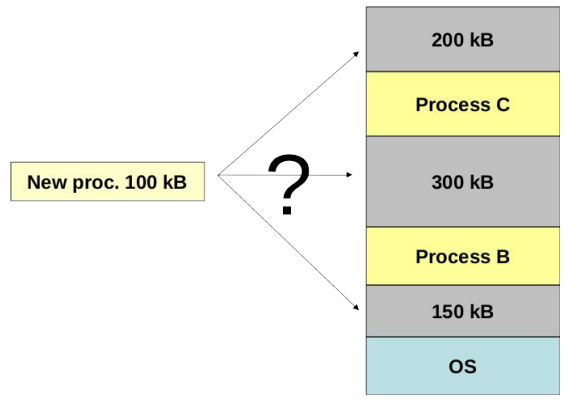
\includegraphics[width = .4\textwidth]{../res/imgs/main memory/allocation_choice.png}
    \caption{In quale allocazione di memoria verrà inserito il nuovo processo?}
    \label{fig:allocation_choice}
\end{figure}

\noindent La scelta può essere effettuata secondo 3 criteri diversi:
\vspace{-5px}
\begin{itemize}
\setlength{\itemsep}{-.15 em}
    \item \textit{First-fit}: il primo posto disponibile viene occupato dal nuovo processo. Per esempio, se abbiamo la memoria ad allocazione variabile e all'interno di essa abbiamo un processo B e un processo C, si va a scorrere la memoria e si inserisce il nuovo processo nel primo \textit{hole} disponibile;
    \item \textit{Best-fit}: in questo caso si cerca di allocare il nuovo processo nella zona il più si avvicina alla dimensione del processo. Di conseguenza, al fine di allocare il processo in memoria è prima necessario scorrerla tutta con una ricerca \textbf{lineare};
    \item \textit{Worst-fit}: infine, con questa tecnica, si sceglie lo spazio con la dimensione peggiore possibile, ovvero la dimensione più grande possibile; ciò significa che il buco lasciato in memoria sarà il più grande possibile. Anche in questo caso è necessario fare una ricerca \textbf{lineare}.
\end{itemize}

% 
\subsubsection{Problema della frammentazione}\label{frammentazione}
Abbiamo ormai constatato che quando si allocano nuovi processi in memoria, questi lasciano in memoria dei buchi che non sempre possono essere riempiti. In particolare, nel caso della partizione fissa (\ref{partizione_fissa}) questo tipo di problema viene chiamato \textbf{frammentazione interna}, questo perché è interna alla partizione in quanto il processo allocato non riesce a riempire pienamente lo spazio della partizione (osservare la figura \ref{fig:fixed_partition}). Questo rappresenta ovviamente un problema perché può essere che in memoria ci sia in totale dello spazio disponibile (ovvero la somma di tutti gli spazi grigi in figura) ma essendo non contiguo non permette un ulteriore inserimento del processo in memoria. 

Alla frammentazione interna si contrappone la \textbf{frammentazione esterna}, che si verifica nel caso dell'allocazione a partizione variabile (\ref{partizione_variaibile}). Facendo appunto riferimento alla figura \ref{fig:variable_partition}, può essere che una volta inserito il processo 9 all'interno della memoria si siano generati due buchi che non sono abbastanza grandi al fine di contenere un altro processo. Si è fatto uno studio dove si è notato che con l'allocazione a partizione variabile e il \textbf{first-fit}, ogni N blocchi in memoria, se ne perdono la metà a causa della frammentazione esterna: di conseguenza all'incirca $1/3$ della memoria è inutilizzato (\textit{50-percent rule}). 

Una soluzione al problema della frammentazione esterna è il \textbf{compacting} (compattazione), illustrata in figura \ref{fig:compacting}. Poniamo che il processo B termini e venga rimosso dalla memoria; si creerebbe un buco sopra e sotto il processo C che non consentirebbe a processi di grandi dimensione di essere inseriti all'interno della memoria.
\begin{figure}[h]
    \centering
    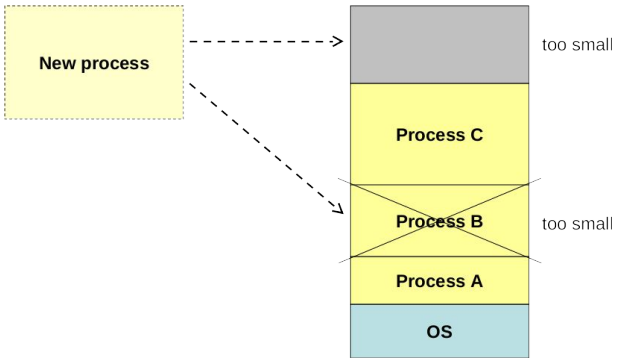
\includegraphics[width = .48\textwidth]{../res/imgs/main memory/compacting1.png}
    \hspace{2em}
    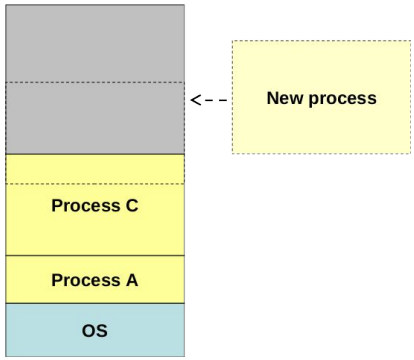
\includegraphics[width = .32\textwidth]{../res/imgs/main memory/compacting2.png}
    \caption{Processo di compacting, una soluzione alla frammentazione esterna.}
    \label{fig:compacting}
\end{figure}
Allora, al posto di lasciare così com'è la memoria, si sceglie di compattare tutti i processi nella parte bassa in memoria al fine di avere un'unica zona di memoria con soli processi (e senza buchi) e una parte in memoria completamente a disposizione dei nuovi processi. Sembrerebbe una soluzione ottimale ma in realtà comporta alcuni diversi problemi. Primo tra tutti è che bisogna capire come \textbf{spostare} dei \textbf{processi} in memoria: fino ad ora venivano inseriti e rimossi ma mai spostati da una zona all'altra. In secondo luogo, se si ripete questo processo per milioni di locazioni in memoria, compattare molti processi diventa un \textbf{problema computazionale} non indifferente, soprattutto se si fa ogni volta che un processo in memoria viene rimosso. È quindi evidente che la soluzione sia tutto fuorché ottimale e che quindi i problemi di frammentazione, con questo tipo di allocazioni, persistono.

% 
\subsection{Paginazione (\textit{paging)}}\label{paginazione}
Ecco quindi che introduciamo questo nuovo tipo di allocazione, molto più moderno ed elegante, ovvero la \textbf{paginazione}. Il concetto alla base di questa tecnica è quello di dividere la memoria in locazioni di dimensione fissa $\overline{n}$, chiamate \textbf{\textit{frames}}, e dividere lo spazio logico dei processi in blocchi della stessa dimensione $\overline{n}$. Generalmente, nei sistemi operativi moderni, $\overline{n}\in [ \texttt{512 Bytes},\texttt{16 MBytes} ]$. In questo modo è quindi possibile dividere i processi in \textbf{pagine} e associare ad ogni pagina di ogni processo in esecuzione un frame in memoria, proprio come illustrato nella figura \ref{fig:paging}.
\begin{figure}[h]
    \centering
    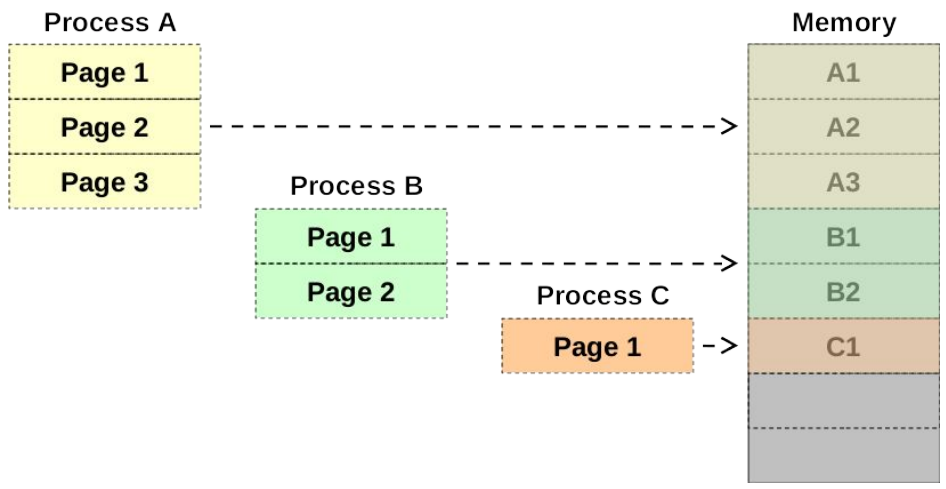
\includegraphics[width = .6\textwidth]{../res/imgs/main memory/paging.png}
    \caption{Il funzionamento ad alto livello della paginazione.}
    \label{fig:paging}
\end{figure}
Questa tecnica risolve subito il problema della frammentazione esterna e dei buchi. Osservando infatti la figura \ref{fig:remove_process_paging}, nel momento in cui il processo B termina l'esecuzione e viene rimosso dalla memoria, dovrebbero rimanere dei buchi tra il processo A e il processo C. Questo buchi però vengono immediatamente colmati dal processo D le quali pagine vengono mappate nei frames che prima erano occupati da B e dal frame seguente al processo C. In questo modo, proprio perché le pagine e i frames sono della stessa dimensione si incastrano perfettamente tra di loro e non lasciano nessun buco.
\begin{figure}[h]
    \centering
    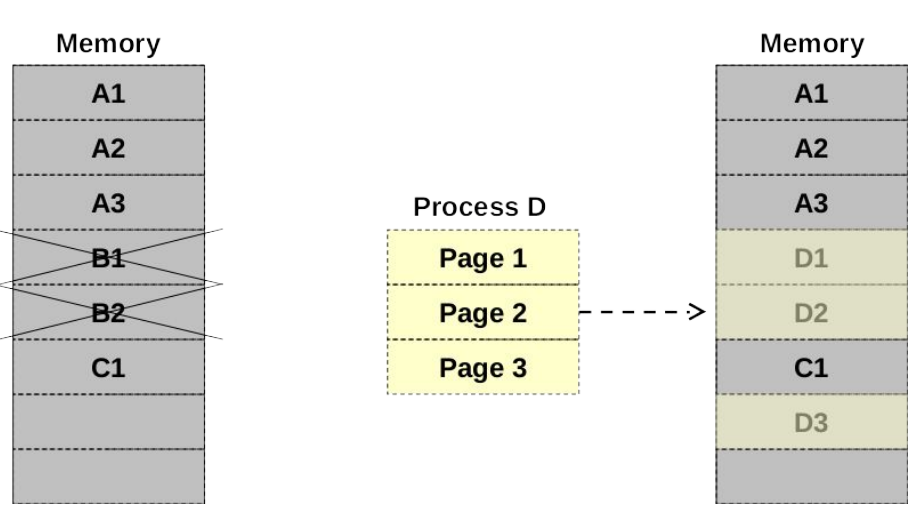
\includegraphics[width = .6\textwidth]{../res/imgs/main memory/remove_process_paging.png}
    \caption{La rimozione di un processo e l'inserimento di un altro con la paginazione.}
    \label{fig:remove_process_paging}
\end{figure}

Se andiamo a dividere lo spazio logico in pagine e la memoria viene divisa in frames, abbiamo bisogno di un supporto che mappa ciascuna pagina del processo ad un frame in memoria. Questo supporto è chiamato \textbf{page table} (discussa approfonditamente nel paragrafo \ref{page_table}) e si occupa appunto della traduzione di indirizzi logici (pagine) in indirizzi fisici (frames). Si osserva che la page table è una struttura associata ad ogni singolo processo. Di conseguenza due processi hanno due page table differenti.

% 
\subsubsection{Frammentazione interna}
Osserviamo infine un'ultima cosa: pur avendo eliminato il problema della frammentazione esterna, la \textbf{frammentazione interna} persiste: molto spesso infatti un processo non avrà esattamente la dimensione di \textit{n} pagine, anzi, avrà generalmente una dimensione che è minore della dimensione occupata da \textit{n} pagine ma comunque più grande di quella occupata da \textit{n-1} pagine. Di conseguenza l'ultima pagina non sarà mai completamente piene ma avrà dello spazio non occupato. Questo spazio non potrà nemmeno essere utilizzato da altri processi dato che come sappiamo la dimensione della pagina è fissa.

Facciamo un esempio per fissare il concetto. Abbiamo un processo di \texttt{10 KBytes} che deve essere allocato in memoria. Poniamo che la dimensione delle pagine (e quindi dei \textit{frames}) è di \texttt{4 KBytes}. Al fine di inserire il processo in memoria sono quindi necessarie 3 pagine, che forniscono uno spazio di \texttt{3 * 4 KBytes = 12 KBytes} che è maggiore rispetto ai \texttt{10 KBytes} del processo: sono quindi sprecati \texttt{12 - 10 = 2 KBytes} che non potranno mai essere occupati da altri processi. Al caso migliore lo spreco è di \texttt{1 Byte} (ovvero la dimensione di 1 cella in memoria), mentre al caso peggiore lo spreco è di \texttt{$\overline{n}$ - 1 Bytes}. È ragionevole affermare che invece al \textbf{caso medio} si spreca indicativamente la metà di un frame.

Una soluzione a cui si potrebbe intuitivamente pensare è quella di ridurre sempre di più la dimensione delle pagine al fine di sprecare sempre meno memoria. Riducendo però la dimensione delle pagine (e quindi dei frame) significa che abbiamo a che fare con un numero maggiore di pagine: se dimezziamo la dimensione di una pagina avremmo quindi il doppio delle pagine da indirizzare: è evidente che più si riduce la dimensione di un frame, la complessità aumenta. La soluzione migliore non è quindi avere delle pagine estremamente piccole ma riuscire a trovare un compromesso tra la dimensione della pagina e la complessità che ne deriva.

% 
\subsubsection*{Calcolo della frammentazione interna}
Un secondo esercizio che può ritornare utile è quello del calcolo della frammentazione interna durante la paginazione. Poniamo di avere la dimensione della pagina di \texttt{2048 Bytes} (e quindi lo spazio per l'offset è di 11 bit) e che la dimensione del processo in esecuzione sia \texttt{72766 Bytes}. Possiamo ora calcolare il numero di pagine occupate dal processo: $72766 / 2048 = 35.53$. Questo risultato ci dice che il numero di pagine completamente riempite sono 35 e che la 36esima verrà utilizzata ma solo in parte generando quindi della frammentazione interna. I byte sprecati sono infatti $(36 \cdot 2048) - 72766 = 962$ bytes inutilizzati. 

% 
\subsubsection{Traduzione degli indirizzi}
Al fine di convertire le pagine del processo in frames in memoria è quindi necessario un processo di traduzione. Tale traduzione è effettuata attraverso un'\textbf{interpretazione} dell'indirizzo logico. In particolare, tale indirizzo è diviso in due parti: la prima parte (\textit{p}), quella dei bit più significativi (ovvero quelli più a sinistra), indica l'indirizzo della pagina mentre la seconda parte (\textit{d}) indica l'\textit{offset} della cella dall'indirizzo della pagina. La page table si occupa di convertire il numero della pagina nel numero del frame in memoria, mantenendo l'offset invariato.

Osserviamo più nel dettaglio questo processo basandoci sull'illustrazione \ref{fig:paging_hardware}. Prima di tutto il processo fornisce l'indirizzo logico, che, come abbiamo appena visto, è composto da due parti. La parte più significativa, \textit{p}, indica il numero della pagina, in particolare rappresenta il numero dell'indice della tabella dove è contenuto il frame.
\begin{figure}[h]
    \centering
    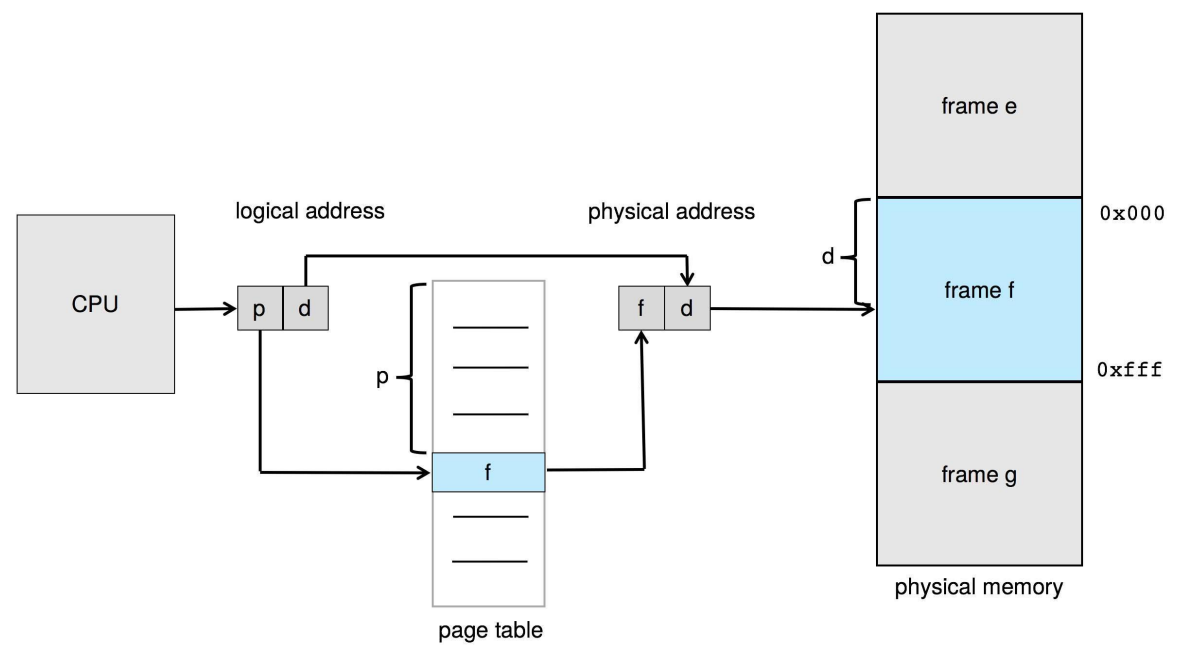
\includegraphics[width = .8\textwidth]{../res/imgs/main memory/paging_hardware.png}
    \caption{Il processo di conversione da indirizzo logico a indirizzo fisico.}
    \label{fig:paging_hardware}
\end{figure}
 Una volta che l'accesso alla page table è stato effettuato, si preleva il frame \textit{f} e lo si sostituisce nell'indirizzo logico che diventa un indirizzo fisico. A questo punto non ci resta che andare in memoria nel frame \textit{f} e aggiungerci l'offset con valore \textit{d}.

% 
\subsubsection*{Calcolo di un indirizzo tradotto}
Supponiamo di avere lo spazio totale di indirizzo logico di $2^{16}$, e quindi un indirizzo logico è 16 bit. Ci viene dato inoltre la grandezza di una pagina, che è 
$2^{12}$. In altre parole, con questa informazione, sappiamo che i bit necessari per l'offset sono 12. A questo punto sappiamo che i bit disponibili per indirizzare le pagine logiche sono $16 - 12 = 4$; di conseguenza abbiamo $2^4 = 16$ pagine logiche disponibili.

A questo punti viene fornito l'indirizzo logico \texttt{0011 0000 1011 1001}. Poniamo inoltre che siamo a conoscenza di tutti i valori presenti nella page table del processo. In quale indirizzo fisico viene mappato l'indirizzo dato? La soluzione è molto semplice: l'indirizzo fornito è ovviamente lungo 16 bit; sappiamo inoltre che durante la conversione vengono modificato solo i bit del numero della pagina, che in questo caso sono i primi quattro verso sinistra, ovvero \texttt{0011}. A questo punto scorriamo sulla page table alla cella numero $0011_2  = 3_{10}$ e scopriamo che la pagina viene mappata nel frame \texttt{1110}. Procediamo quindi con una banale sostituzione, ottenendo l'indirizzo fisico di valore: \texttt{1110 0000 1011 1001}. L'illustrazione \ref{fig:paging_example} è esemplificativa di questo processo.
\begin{figure}[h]
    \centering
    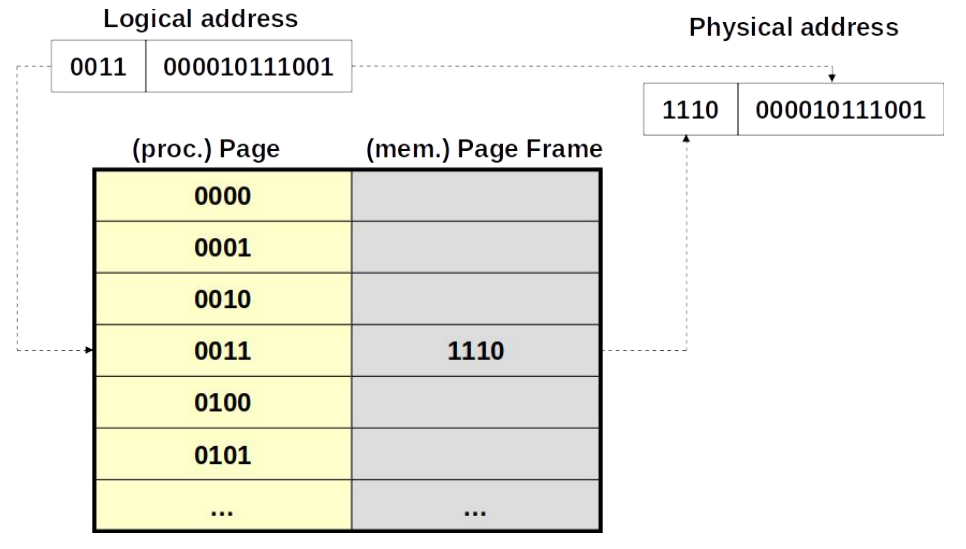
\includegraphics[width = .5\textwidth]{../res/imgs/main memory/paging_example.png}
    \caption{Esempio di una paginazione.}
    \label{fig:paging_example}
\end{figure}

% 
\subsubsection{Allocazione nei frames liberi}
Nel momento in cui si carica un nuovo processo in memoria, i frames che devono essere riempiti sono, naturalmente, quelli vuoti. Questi sono presenti in una lista (la \textbf{free-frame list}) che è detenuta dal sistema operativo al fine di tenere traccia dei frames disponibili. Di conseguenza quando deve essere inserita una pagina in memoria, il sistema operativo prende un frame disponibile dalla free-frame list che viene associato alla pagina. Questa associazione viene quindi inserita nella page table del processo. Nella figura \ref{fig:free-frame_allocation} è illustrato questo processo. Inizialmente arriva un nuovo processo che contiene 4 pagine. Queste 4 pagine, in quanto nuove non hanno ad esse associato in frame, e di conseguenza non sono presenti nemmeno sulla tabella delle pagine.
\begin{figure}[h]
    \centering
    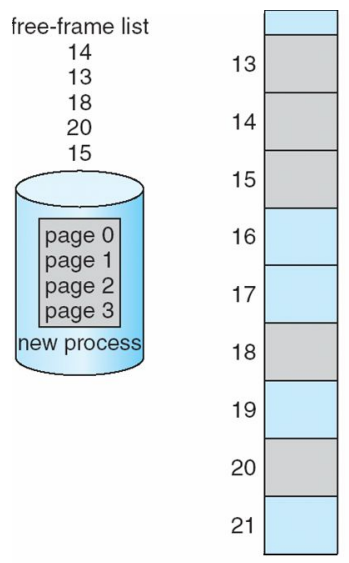
\includegraphics[width = .2\textwidth]{../res/imgs/main memory/before_allocation.png}
    \hspace{6em}
    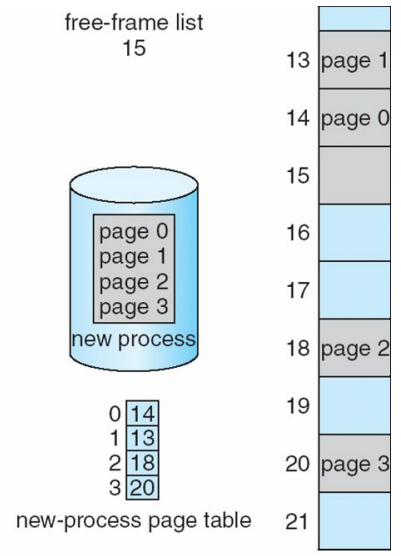
\includegraphics[width = .235\textwidth]{../res/imgs/main memory/after_allocation.png}
    \caption{Il processo di allocazione delle pagine in nuovi frames liberi.}
    \label{fig:free-frame_allocation}
\end{figure}
Di conseguenza, nel momento in cui la richiesta viene accettata dal sistema operativo, alle 4 pagine vengono associati 4 frames liberi che erano presenti nella lista. Dopo l'allocazione infatti notiamo che i frame che erano liberi ora contengono le 4 pagine e non sono più presenti nella free-frame list. Ancora più importante è però notare che nella pagina delle tabelle del processo si sono aggiunte le nuove associazioni.

% 
\subsection{Page table}\label{page_table}
Entriamo ora più nel dettaglio, e discutiamo in maniera più approfondita la, ormai nota, tabella delle pagine. Come sappiamo questa tabella non è unica in tutto il sistema operativo ma è presente una page table per ogni processo. Tipicamente la tabella ha dimensioni così significative che essa stessa è mantenuta in memoria. Quindi per ogni processo in esecuzione, esiste una sua page table associata che è presente in memoria. In particolare, della page table, il sistema operativo tiene traccia di due importanti valori (vedi figura \ref{fig:page_table_registers}), al fine di riuscire ad associare ogni processo alla sua tabella:
\vspace{-5px}
\begin{itemize}
\setlength{\itemsep}{-.15 em}
    \item \textit{Page-Table Base Register} (\textbf{PTBR}), che contiene l'indirizzo alla prima cella in memoria da cui parte la tabella;
    \item \textit{Page-Table Length Register} (\textbf{PTLR}), che si occupa di immagazzinare la lunghezza della tabella in memoria. 
\end{itemize}
Ovviamente, nel momento in cui avviene un \textit{context switch} (vedi paragrafo \ref{context_switch}), i due registri vengono modificati. In questo modo si è in grado di associare ad ogni processo la sua personale page table.
\begin{figure}[h]
    \centering
    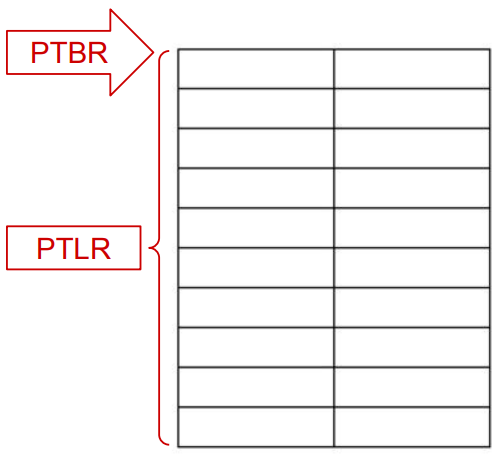
\includegraphics[width = .3\textwidth]{../res/imgs/main memory/page_table_registers.png}
    \caption{I due registri necessari per tenere traccia della page table in memoria.}
    \label{fig:page_table_registers}
\end{figure}

% 
\subsubsection{Translation Look-aside Buffer (TLB)}
Il problema di avere una tabella in memoria è che per accedere ad un indirizzo fisico in memoria, è necessario effettuare due accessi in memoria:
\vspace{-4px}
\begin{enumerate}
\setlength{\itemsep}{-1px}
    \item Accesso alla page table in memoria per tradurre l'indirizzo logico in un indirizzo fisico;
    \item Accedere alla locazione dell'indirizzo fisico fornito dalla tabella delle pagine.
\end{enumerate}
Così facendo il tempo per accedere ad un frame in memoria è raddoppiato. La soluzione a questo problema è fornita dalla \textbf{TLB}, che è una speciale \textbf{cache} la quale mantiene la porzione della page table che è usata più spesso. In questo modo la CPU non deve sempre accedere alla memoria bensì accede alla TLB che è molto più rapida e quindi consente di risparmiare tempo. Questa cache è infatti implementata fisicamente a livello di CPU e i suoi tempi di accesso sono estremamente ridotti comparati a quelli della memoria. Si osserva inoltre che, se la velocità di accesso è elevata, lo spazio di memorizzazione è molto basso: generalmente infatti le TLB contengono dalle 64 alle 1024 righe.

Ora che abbiamo inserito la TLB nel processo di traduzione da pagina logica a fisica, vediamo come questo è cambiato. L'illustrazione \ref{fig:paging_hardware_TLB} rappresenta l'intero processo di traduzione.
\begin{figure}[h]
    \centering
    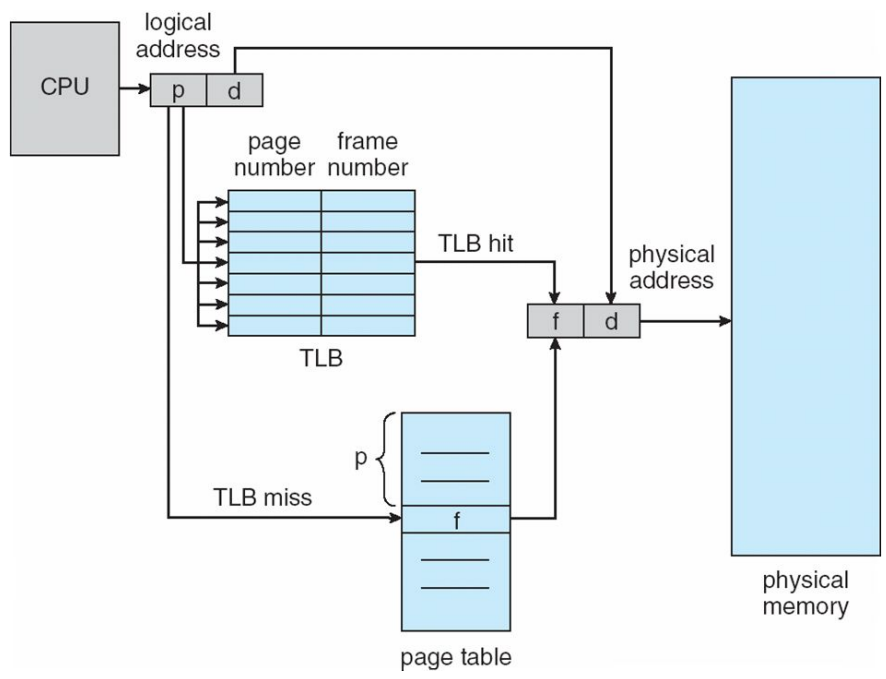
\includegraphics[width = .7\textwidth]{../res/imgs/main memory/paging_hardware_TLB.png}
    \caption{Il processo di traduzione effettuato con l'ausilio della TLB.}
    \label{fig:paging_hardware_TLB}
\end{figure}
Una volta che arriva l'indirizzo logico dalla CPU si andrà innanzitutto a controllare se il numero della pagina logica è presente all'interno della TLB. Nel caso sia presente, si ha un \textbf{TLB hit} e si ottiene subito il frame associato alla pagina; di conseguenza si può subito accedere in memoria. Si osserva che la verifica della pagina all'interno della TLB viene effettuata in \textbf{parallelo}, di conseguenza tale verifica è praticamente istantanea. Se invece la pagine non è presente nella TLB, si verifica il cosiddetto \textbf{TLB miss}. A questo punto è necessario effettuare un primo accesso in memoria al fine di trovare il frame nella page table e, dopo di che, effettuare un secondo accesso al frame allocato. 

Va inoltre specificato che a differenza delle page table, la TLB è una unica per tutta il sistema ed è quindi "condivisa" da tutti i processi. Di conseguenza è presente un identificativo, chiamato \textit{address-space identifier} (\textbf{ASID}), che indica se la particolare entry della TLB fa parte o meno del processo che ne fa richiesta. Questo identificativo serve per fare in modo che i processi accedano solo nei loro indirizzi. Se questa funzionalità non fosse implementata, una soluzione comunque lecita è quella di resettare la TLB ogni volta che un context switch (\ref{context_switch}) si genererebbe però dell'overhed.

Si osserva infine che è anche possibile far si che alcune entry rimangano permanentemente dentro la TLB in quanto, magari, sono delle pagine che vengono richieste quasi sempre. In questo caso si parla infatto di \textit{wired down entries}.
% 
\subsubsection*{Analisi delle performance con la TLB}
Definizmo che \textbf{hit ratio} la percentuale secondo la quale si ha un TLB hit. Poniamo di avere un hit ratio di \texttt{80\%}: 80 volte su 100 si verificherà un TLB hit. Supponiamo inoltre che il tempo di accesso alla memoria sia 10 ns (nanosecondi). Da queste informazioni possiamo evincere che se si ha un TLB hit, il tempo di accesso sarà 10 ns, altrimenti il tempo di accesso si duplicherà diventando 20 ns. A questo punto è possibile calcolare l'\textbf{EAT}, ovvero \textit{Effective Access Time}:
\begin{gather*}
    \text{EAT} = 0.8 \cdot 10 + 0.2 \cdot 20 = 12\text{ ns}
\end{gather*}
Passando però ad un hit ratio più realistico, \texttt{99\%}, il tempo effettivo di accesso diventa:
\begin{gather*}
    \text{EAT} = 0.99 \cdot 10 + 0.01 \cdot 20 = 10.1\text{ ns}
\end{gather*}

% 
\subsubsection{Bit di validità}
Uno dei meccanismi dedicati alla protezione della memoria è quello di implementare un bit di validità, chiamato \textbf{valid-invalid} bit. Alla page table viene aggiunta una colonna che contiene tale bit di validità. In questo modo, ogni entry della page table avrà un bit che indicherà se quell'associazione sia valida o meno. In particolare il bit si occupa di segnalare se la pagina si trova nello spazio di indirizzi logici del processo. Osservando la figura \ref{fig:valid-invalid_bit}, notiamo che all'interno della page table le pagine 6 e 7 sono invalide proprio perché non sono presenti nello spazio di indirizzi del processo (che si ferma alla quinta pagina).
\begin{figure}[h]
    \centering
    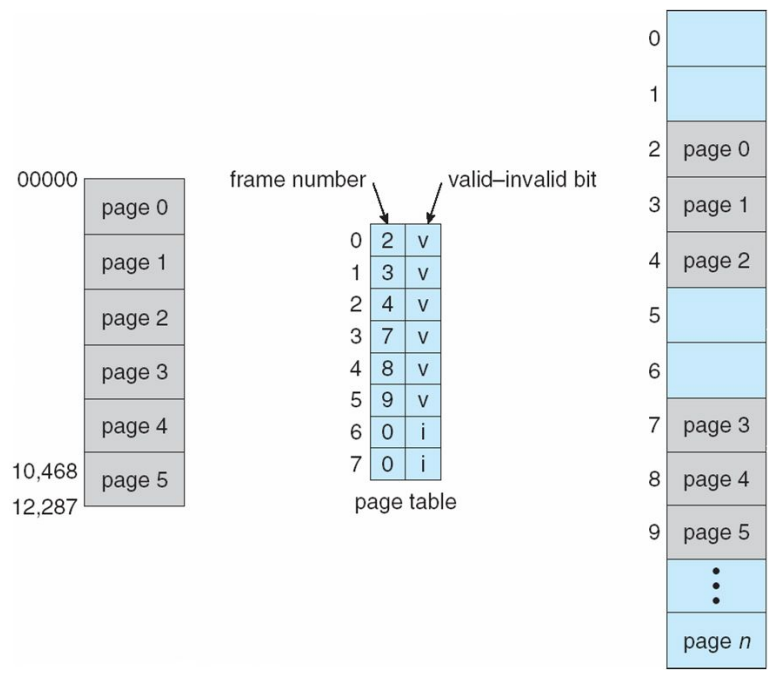
\includegraphics[width = .6\textwidth]{../res/imgs/main memory/valid-invalid_bit.png}
    \caption{Implementazione del valid-invalid bit sulla tabella delle pagine.}
    \label{fig:valid-invalid_bit}
\end{figure}

% 
\subsubsection*{Il problema delle macchine moderne}
La page table inserita in maniera continua in memoria con l'ausilio della TLB sembra una soluzione ottima. E lo era un tempo, quando gli indirizzi erano al più di 16 bit. Con l'avvento però di indirizzi da 32 e 64 bit la situazione è però peggiorata perchè la dimensione delle pagine è però sempre la stessa e non può cambiare. Poniamo di avere delle pagine da 4KB, che quindi necessitano di 12 bit per l'indirizzamento, rimangono 32 - 12 = 20 bit per indirizzare tutte le pagine. Ciò significa che è possibile avere fino a $2^{20}$ pagine da indirizzare, ovvero avere una tabella con più di un milione di righe. Nei casi ancora più moderni, quando si ha a che fare con indirizzi da 64 bit, si ha la possibilità di avere $2^{52} \approx 4\cdot10^{15}$ ovvero 4 biliardi di pagine. 

Ricordiamo che alla base della paginazione c'è la necessità di non dover allocare in maniera continua nulla in memoria, di conseguenza è giusto che anche la page table abbia lo stesso trattamento. Ecco quindi che nascono diverse tecniche al fine di riuscire a spezzettare anche la page table all'interno della memoria. 

% 
\subsubsection{Page table gerarchica}
La prima soluzione che si è pensata è quella di creare una page table che indirizzi un altro numero di page tables che a loro volta indirizzano i frames in memoria, proprio come rappresentato nell'illustrazione \ref{fig:hierarchical_page_table}.
\begin{figure}[h]
    \centering
    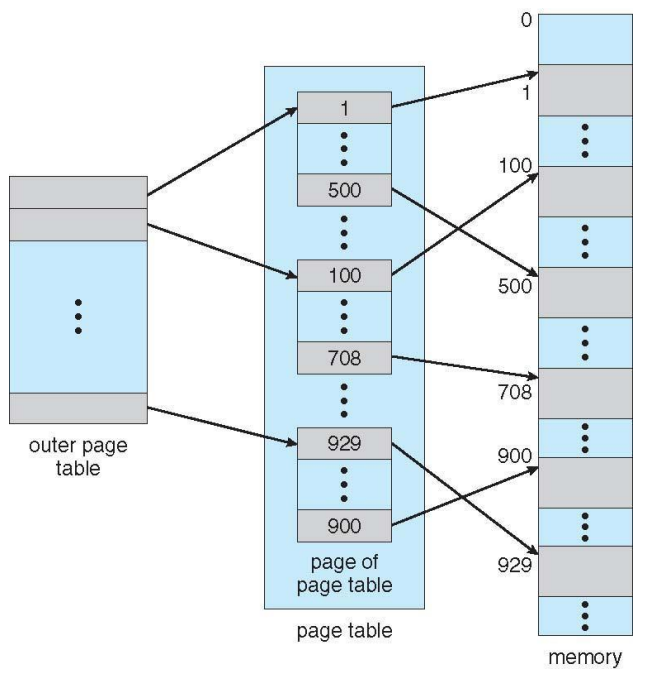
\includegraphics[width = .45\textwidth]{../res/imgs/main memory/hierarchical_page_table.png}
    \caption{Struttura gerarchica della page table.}
    \label{fig:hierarchical_page_table}
\end{figure}
Come cambia ora il processo di traduzione tra una pagina e un frame? Partiamo da un indirizzo a 32 bit e poniamo che le pagine abbiano la dimensione di 4 KB e che quindi necessitino di 12 bit per essere indirizzati (\textit{d}). A questo punto i restanti 20 bit vengono a loro volta divisi in due parti: la prima parte $p_1$ punta ad un elemento della \textit{outer page table} e la seconda parte $p_2$ punta ad un elemento della tabella puntata da $p_1$ (figura \ref{fig:hierarchical_page_table_access}).
\begin{figure}[h]
    \centering
    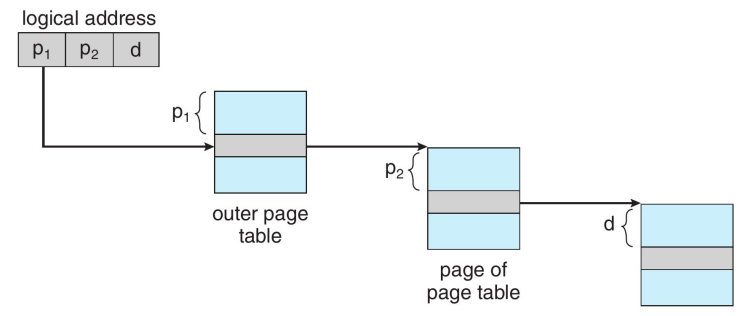
\includegraphics[width = .6\textwidth]{../res/imgs/main memory/hierarchical_page_table_access.png}
    \caption{L'accesso in memoria attraverso una struttura gerarchica della page table.}
    \label{fig:hierarchical_page_table_access}
\end{figure}
In questo modo però puntualizziamo che, senza l'ausilio di una TLB cache, al fine di raggiungere un frame in memoria è necessario fare ben 3 accessi ad essa, triplicando così il tempo necessario per accedere al frame. 

Nelle architetture a 64 bit invece le soluzioni possono essere 2. Avendo 52 bit a disposizione si sceglie di creare una \textit{outer page table} molto grande, indirizzata con 42 bit, e delle tabelle di secondo livello indirizzate da 10 bit. Una seconda soluzione può essere invece l'inserimento di un terzo livello di page table (\textbf{three-level paging scheme}) dove, per esempio, si ha l'outer page table indirizzata con 32 bit, e la tabella secondaria e terziaria indirizzate con 1 bit ciascuna. Si osserva che in questo caso il numero di accessi in memoria quadruplica al fine di accedere ad un frames. Proprio perché la struttura gerarchica non si presta molto bene ad architetture con indirizzi maggiori di 32 bit, si sono progettate altre soluzioni.

% 
\subsubsection{Page table con tabella \textit{hash}}
Al fine di provare a risolvere il problema che è emerso utilizzando una struttura gerarchica si è pensato di implementare una \textbf{\textit{hashed} page table}: ciò significa convertire il numero della pagina attraverso una \textit{hash function} che restituisce una chiave. Tale chiave è l'indice di una tabella che contiene il frame che stiamo cercando. Questo meccanismo è illustrato in modo chiaro nella figura \ref{fig:hashed_page_table} sottostante. 
\begin{figure}[h]
    \centering
    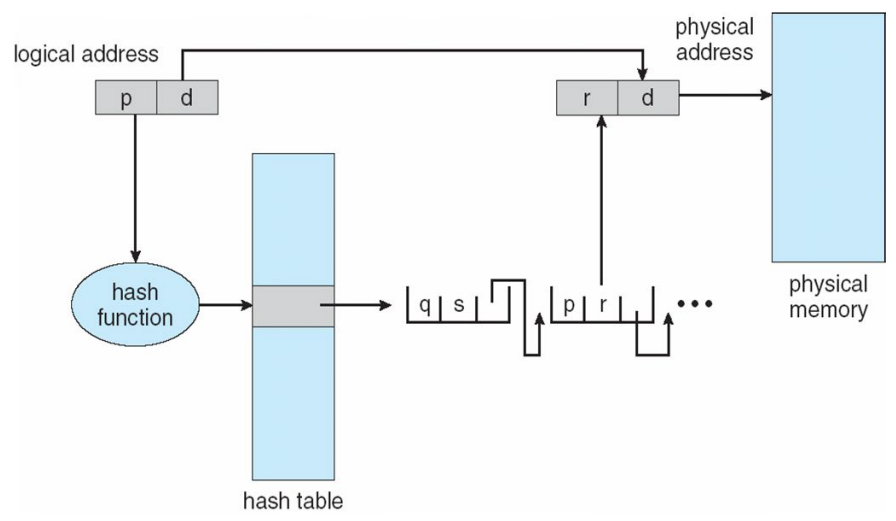
\includegraphics[width = .7\textwidth]{../res/imgs/main memory/hashed_page_table.png}
    \caption{Accesso alla memoria tramite una page table implementata attraverso una hash table.}
    \label{fig:hashed_page_table}
\end{figure}
La \textit{hash table}, a seconda del range delle chiavi fornito, può essere infatti di dimensione molto ridotta. Ricordiamo inoltre che la hash function per valori di pagine diverse può restituire le stesse chiavi: proprio per questo motivo ad ogni entry della hash table in realtà è presente una lista concatenata che contiene tutte le entry che hanno avuto una collisione. Nel caso della figura \ref{fig:hashed_page_table}, il valore della pagina \textit{p} era situato alla seconda posizione della lista. 

Introduciamo anche la \textbf{\textit{clustered} page tables} che è una struttura più moderna e migliorata rispetto alla \textit{hashed page table}. In questa struttura, ogni entry della page table, non corrisponde ad una pagina bensì ad un \textbf{cluster} di frames, che può arrivare fino a 16. In questo modo è possibile fare riferimento a frmaes che possono essere sparsi all'interno della memoria. Così facendo i casi con frames sparsi in diverse locazioni sono più facilmente gestibili.Questa struttura è quindi più efficiente rispetto alla classica implementazione con la tabella hash.
\begin{figure}[h]
    \centering
    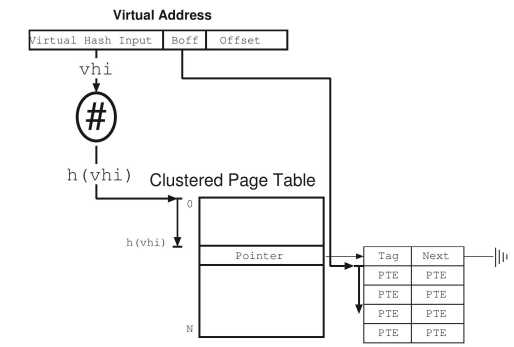
\includegraphics[width = .5\textwidth]{../res/imgs/main memory/clustered_page_table.png}
    \caption{Rappresentazione di una \textit{clustered} page table.}
    \label{fig:clustered_page_table}
\end{figure}

% 
\subsubsection{Page table invertita}
Una terza soluzione è la cosiddetta tabella delle pagine invertita. Fino ad ora abbiamo detto che ogni processo ha la sua propria tabella delle pagine. Questo è necessario perché ogni processo ha il suo indirizzamento logico a cui può corrispondere un insieme di frames nella memoria. Il problema è che generalmente lo spazio di indirizzo logico non è mai utilizzato completamente. Questo perché tipicamente diverse entry all'interno della page table del processo sono invalide e quindi inutilizzate, ma sono comunque presenti.

Allora perché non fare l'opposto? Invece di avere tante tabelle, di notevoli dimensioni che puntano a frames fisici, si è scelto di utilizzare una \textbf{tabella unica} che è indicizzata dai frames fisici reali, e contiene all'interno di ogni elemento la pagina che il frame contiene. Ciò significa che al posto di avere tante tabelle, una per ogni processo, ci ritroviamo con un'unica tabella dove saranno contenuti i frames della memoria fisica e le pagine corrispondenti al processo. Inoltre, nella tabella, sarà necessario aggiungere, per ogni pagina, il numero identificativo del processo, il \texttt{pid}, visto nel capitolo \ref{processes}, altrimenti non si riuscirebbe a risalire a quale processo appartiene quella pagina. Possono infatti essere presenti due pagine logiche \texttt{0110}, ma una appartiene al processo 314 e l'altra magari appartiene al processo 159.
\begin{figure}[h]
    \centering
    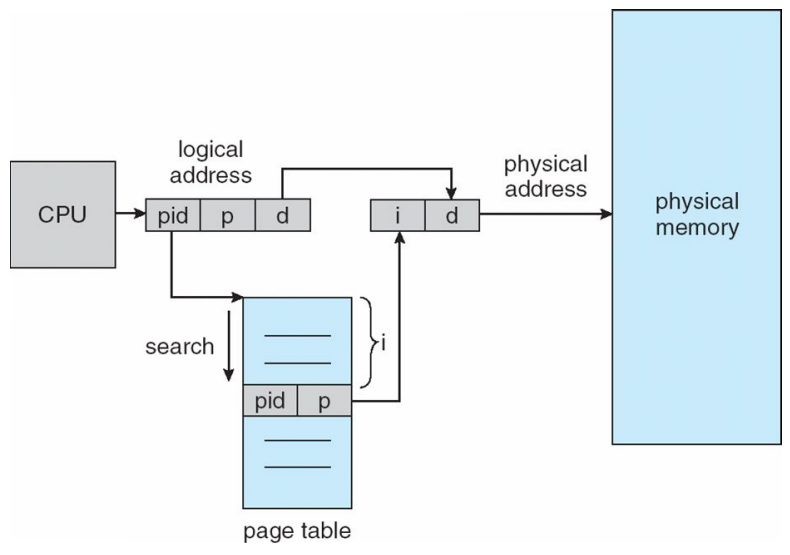
\includegraphics[width = .6\textwidth]{../res/imgs/main memory/inverted_page_table.png}
    \caption{Accesso in memoria attraverso la tabella delle pagine invertita.}
    \label{fig:inverted_page_table}
\end{figure}

\noindent La figura \ref{fig:inverted_page_table} mostra il procedimento necessario per accedere ad un frame in memoria. Prima di tutto è necessario effettuare una \textbf{ricerca} sulla tabella invertita l'identificativo del processo (\texttt{pid}) e la pagina cercata. Se tale ricerca ha buon fine allora il frame in memoria è presente ed è quindi possibile effettuare l'accesso.

Discutiamo, infine, alcuni vantaggi e svantaggi della tabella delle pagine invertita. Il vantaggio più evidente è che lo spazio occupato dalla tabella invertita è nettamente minore rispetto alla somma dello spazio occupato da ciascuna tabella per i processi in esecuzione. D'altro canto però il tempo di \textbf{ricerca lineare} nella tabella invertita genera dell'overhed. Questo però può essere ridotto implementato una tabella di hash per limitare la ricerca all'interno della tabella invertita. È inoltre possibile migliorare le prestazione tramite l'ausilio della TLB cache.

% 
\subsection{Swapping}\label{swapping}
Per quanto il metodo per paginare la memoria sia efficiente, ci saranno sempre dei casi in cui è necessario rendere dello spazio disponibile in memoria, rimuovendo uno o più processi. Introduciamo ora una tecnica che serve proprio per questo, si chiama \textit{swapping} (su disco o, in generale, sul \textit{backing store}), che è il procedimento secondo il quale si prende un processo dalla memoria e lo si salva temporaneamente sul disco rigido. Immaginiamo di avere in memoria 100 processi ed aver esaurito lo spazio. per aggiungere il 101 esimo è necessario per forza rimuovere dei processi. Si sceglie infatti di prendere quei processi che sono in attesa (per esempio di un I/O) e che sono fermi in memoria e portarli sul disco, proprio come illustrato nella figura \ref{fig:swapping}.
\begin{figure}[h]
    \centering
    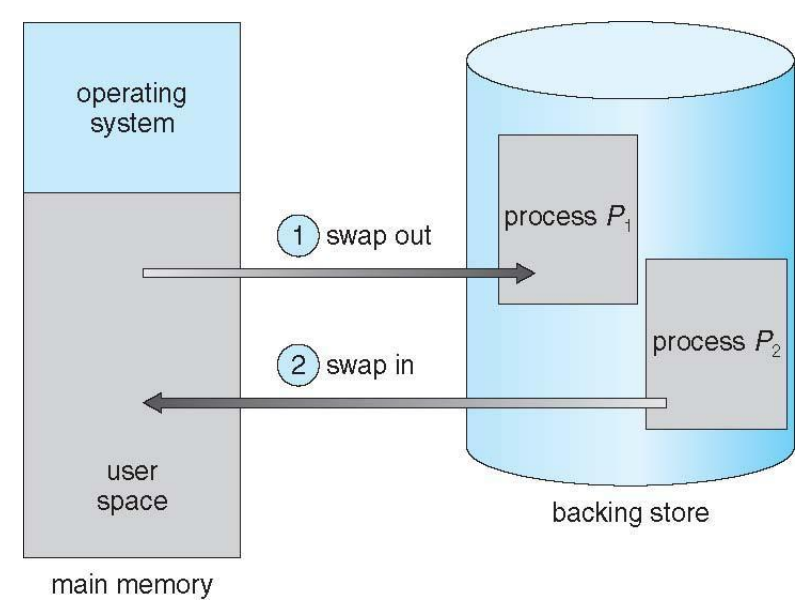
\includegraphics[width = .45\textwidth]{../res/imgs/main memory/swapping.png}
    \caption{Processo di \textit{swap-in} e \textit{swap-out} dal backing store.}
    \label{fig:swapping}
\end{figure}
Il tempo di \textit{swap-in} e \textit{swap-out} rimane comunque un tempo significativo dato che il backing store è una memoria ad alta capacità ma molto lenta. È quindi necessario tenere conto anche del \textbf{tempo di trasferimento} nel momento in cui si scambiano i processi. Ovviamente sarà presente anche una \textbf{ready-queue} che contiene tutti i processi presenti nel disco che non sono più in attesa di un evento e che sono quindi pronti per essere inseriti in memoria. Naturalmente al tempo di trasferimento del processo \textit{in / out} dal disco va sommato anche il tempo necessario per effettuare il context switch (\ref{context_switch}), ovvero ricaricare lo stato del processo nella CPU.

Sono presenti anche delle varianti dello swapping, dove si va a scegliere quale processo portare fuori in base alla priorità: è un concetto molto simile allo scheduling con priorità che abbiamo visto nel paragrafo \ref{priority scheduling}.

% 
\subsubsection{Swapping con paginazione}
Lo swapping classico, tipicamente non è più utilizzato nei sistemi operativi moderni. Spesso infatti non si fa lo swapping dell'intero processo ma solamente di alcune pagine di quel processo. Ecco quindi che parliamo di \textit{swapping with paging}, rappresentato in figura \ref{fig:swapping_with_paging}. La scelta delle pagina da rimpiazzare sarà delegata agli algoritmi di \textit{page replacement} (vedi paragrafo \ref{page replacement}).
\begin{figure}[h]
    \centering
    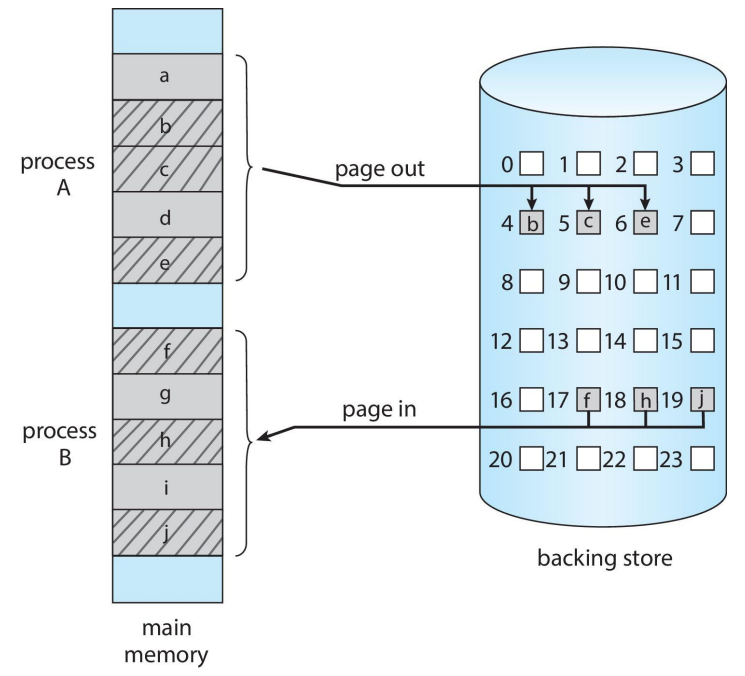
\includegraphics[width = .5\textwidth]{../res/imgs/main memory/swapping_with_paging.png}
    \caption{Rappresentazione del processo di swapping solo su determinata pagine di un processo.}
    \label{fig:swapping_with_paging}
\end{figure}

% 
\subsubsection{Swapping nei dispositivi mobili}
Nei sistemi operativi per \textit{mobile devices} la questione è un po' più complicata in quanto effettuare uno swapping è molto dispendioso, sia da un punto di vista energetico, ma soprattutto perché i supporti di memorizza dei dispositivi mobili spesso hanno un numero limitato di accessi in scrittura e dopo di chè le performance diminuire. Di conseguenza si cerca sempre di evitare la scrittura sul backing store.

Sono presenti ovviamente dei metodi alternativi. Per esempio \textbf{iOS} al fine di liberare memoria domanda a dei processi in esecuzione se qualcuno può volontariamente rilasciare la memoria altrimenti può forzatamente terminare un processo in esecuzione. D'altra parte, \textbf{Android} sceglie di terminare applicazioni che generalmente sono dormienti o in background. Nel momento in cui l'applicazione è terminata lo stato dell'applicazione viene comunque memorizzato al fine di essere già pronta per ripartire.  

% 
\subsection{Segmentazione (\textit{segmentation})}
Introduciamo ora un nuovo modello di allocazione della memoria che è tuttora utilizzato ma non è tanto diffuso quanto la paginazione: stiamo parlando della segmentazione. Quando abbiamo parlato della paginazione, avevamo più volte specificato che la dimensione della pagina è fissa. Nel \textit{segmentation} invece noi permettiamo che la dimensione sia variabile. Non parliamo delle pagine che hanno la stessa dimensione, ma di \textbf{segmenti} di dimensione variabile. Osservando la figura \ref{fig:segmentation}, notiamo che i processi sono appunto divisi in segmenti di dimensione variabile.
\begin{figure}[h]
    \centering
    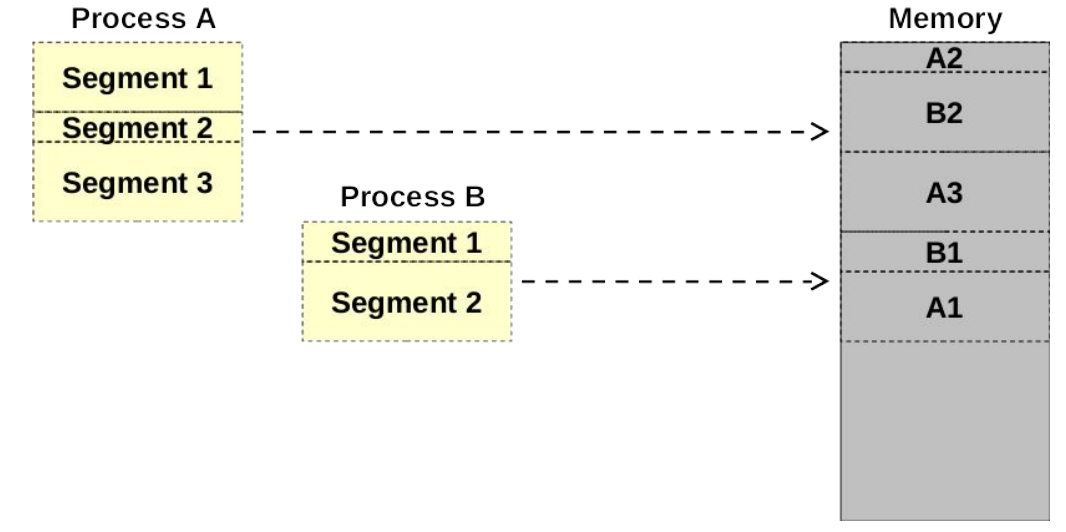
\includegraphics[width = .6\textwidth]{../res/imgs/main memory/segmentation.png}
    \caption{Il funzionamento ad alto livello della segmentazione.}
    \label{fig:segmentation}
\end{figure}
La dimensione di un segmento è decisa in base all'organizzazione e alla logica del programma stesso: potrebbe essere che alcuni segmenti contengono il \texttt{main}, altri contengono delle librerie, altri ancora che contengono le variabili. 

\subsubsection{Segment table}
Al fine di tener traccia di questi segmenti non è più necessaria una tabella della pagine, bensì una \textbf{tabella dei segmenti}. Questa contiene tre campi:
\vspace{-4px}
\begin{enumerate}
\setlength{\itemsep}{-1px}
    \item I primi bit dell'indirizzo logico corrispondono al \textbf{numero di segmento};
    \item La \textbf{dimensione} del segmento che si trova in memoria;
    \item L'indirizzo della prima cella del segmento, ovvero il \textbf{base address}.
\end{enumerate}

Osserviamo la figura \ref{fig:segment_table} e discutiamo nel dettaglio il processo di traduzione da un indirizzo logico ad uno fisico. Quando un indirizzo logico viene fornito, questo è diviso in due parti: il numero del segmento e l'offset.
\begin{figure}[h]
    \centering
    \hspace{6.5 em}
    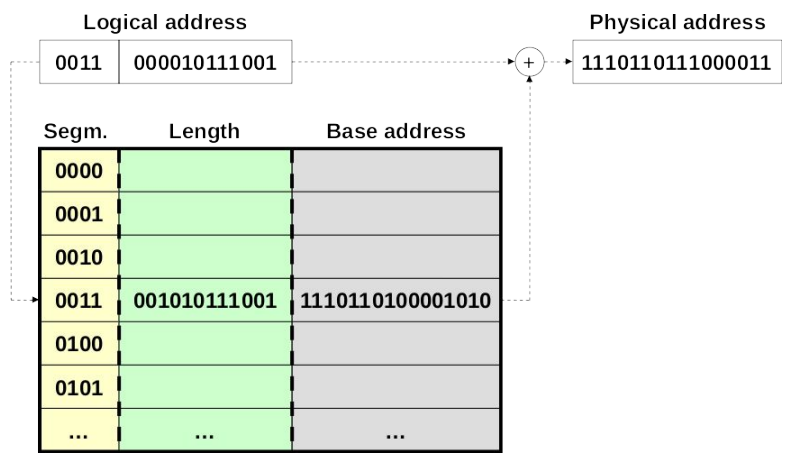
\includegraphics[width = .6\textwidth]{../res/imgs/main memory/segment_table.png}
    \caption{processo di traduzione di un indirizzo logico a fisico mediante la segment table.}
    \label{fig:segment_table}
\end{figure}
A questo punto si prendo il numero del segmento, che è l'indice della segment table. A questo punto si controlla che l'offset sia minore della dimensione del segmento in memoria, in modo tale da garantire che il processo non invada celle di altri processi. Una volta che la verifica è andata a buon fine, se prende l'indirizzo base e lo si \textbf{somma} con l'offset in modo da ottenere l'indirizzo in memoria del segmento. Si ricorda che nella paginazione il frame veniva concatenato con l'offset, qui invece si somma l'offset all'indirizzo base.

% 
\subsubsection{Modello ibrido}
In molti casi è preferibile combinare la paginazione con la segmentazione. Si va così a creare un \textbf{page-segmented system}. Osservando la rappresentazione \ref{fig:page-segmented_system}, cerchiamo di capire come questi tipi di sistemi funzionino. Innanzitutto l'indirizzo logico (virtuale) è diviso in tre parti: la prima indicizza la segment table, il secondo indicizza la page table e il terzo invece rappresenta l'offset. Inizialmente, quando arriva l'indirizzo logico, si accede alla segment table: al suo interno è contenuto l'indirizzo iniziale della page table.
\begin{figure}[h]
    \centering
    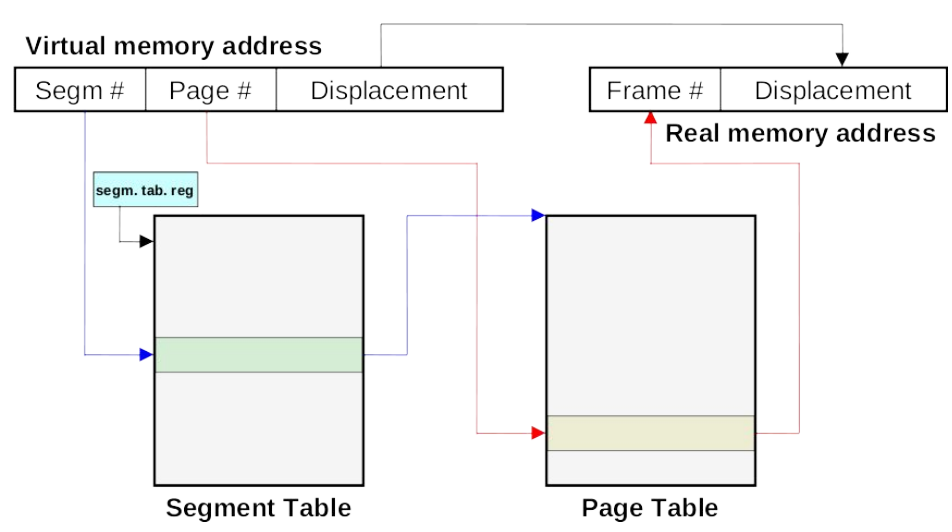
\includegraphics[width = .7\textwidth]{../res/imgs/main memory/page-segmented_system.png}
    \caption{Rappresentazione di un modello che combina paginazione e segmentazione.}
    \label{fig:page-segmented_system}
\end{figure}
A questo punto, utilizzando la seconda parte dell'indirizzo logico si accede alla riga della tabella che contiene l'indirizzo del frame in memoria. Questo frame va quindi concatenato con l'offset.

